\documentclass[a4paper,9pt,french]{scrartcl}
\usepackage[T1]{fontenc}
\usepackage{array}
\usepackage{titlesec}
\usepackage{ulem}
\usepackage[dvipsnames]{xcolor}
\usepackage{color}
\usepackage{babel}
\usepackage{graphicx}
\usepackage[utf8]{inputenc}
\usepackage{geometry}
\usepackage{tikz}
\usepackage{fancyhdr}
\usepackage{hyperref}
\usepackage{caption}
\usepackage{float}
\usepackage{multicol}
\usepackage{amsmath}
%À faire : incertitudes
\geometry{vmargin=2.5cm, a4paper}

\captionsetup{labelfont=sc}
\def\frenchtablename{Tableau}
\pagestyle{fancy}
\renewcommand\headrulewidth{1pt}
\fancyhead[L]{TP 1 - Thermodynamique}
\fancyhead[R]{Saux Paulhenry}

% ----------- Commandes de couleur du modèle ----------
\makeatletter
\newcommand{\coloruline}[2]{%
        \UL@protected\def\temp@uline{\leavevmode \bgroup
            \markoverwith{\textcolor{#1}{\rule[-0.5ex]{2pt}{0.4pt}}}%
        \ULon}%
        \temp@uline{#2}%
    }
\newcommand{\coloruuline}[2]{%
        \UL@protected\def\temp@uuline{\leavevmode \bgroup
            \UL@setULdepth
            \ifx\UL@on\UL@onin \advance\ULdepth2.8\p@\fi
            \markoverwith{\textcolor{#1}{\lower\ULdepth\hbox
                {\kern-.03em\vbox{\hrule width.2em\kern1\p@\hrule}\kern-.03em}}}%
        \ULon}%
        \temp@uuline{#2}%
    }
\makeatother

\renewcommand{\thesection}{\arabic{section}}
\renewcommand{\thesubsection}{\arabic{subsection}}

% ---------------- Modification des titres --------------------
\titleformat{\section}{\Large}{\coloruuline{red}{\thesection. }}{0ex}{\coloruuline{red}}[]
\titleformat{\subsection}{\Large}{\coloruline{red}{\thesection.\thesubsection. }}{0ex}{\coloruline{red}}[]
\titleformat{\subsubsection}{\large}{\coloruline{ForestGreen}{\thesection.\thesubsection.\thesubsubsection. }}{0ex}{\coloruline{ForestGreen}}[]

\begin{document}
\section{Introduction}
\subsection{Objectifs}
\begin{itemize}
    \item Étudier le lien entre la variation d'énergie d'un gaz et ses variables d'état ($P, V, T$).
    \item Appliquer le premier principe de la thermodynamique pour relier les échanges d'énergie ($Q, W$) aux variations d'énergie interne $\Delta U$ et d'enthalpie $\Delta H$.
    \item Déterminer expérimentalement les capacités thermiques molaires $C_v$ et $C_p$ de l'air.
\end{itemize}
\section{Protocole}
\subsection{Matériel}
\begin{itemize}
    \item Ballon en verre de volume $V_0 = 13,4$ L.
    \item Manomètre à tube incliné (diamètre interne $D = 4$ mm).
    \item Système de chauffage (filaments de nickel), alimentation et compteur universel.
    \item Multimètres (mesure de $U$ et $I$) et baromètre (pression atmosphérique).
\end{itemize}

\subsection{Description du montage expérimental}
Le gaz est enfermé dans un vase dont on peut faire varier la pression et le volume via un chauffage par effet Joule. La variation de volume est visualisée par le déplacement d'un liquide dans un manomètre, ce qui induit une légère variation de volume $\Delta V$.

\subsection{Mesures à effectuer}

\begin{enumerate}
    \item \textbf{Préparation du manomètre :} 
    \begin{itemize}
        \item Ouvrir le robinet avec délicatesse pour relier le ballon à l'atmosphère.
        \item Utiliser la seringue pour faire monter le liquide jusqu'à la graduation maximale afin de mouiller les parois et limiter les effets capillaires.
        \item Déconnecter la seringue et attendre l'équilibre (retour au zéro ou à la valeur $\Delta p_{cap}$).
    \end{itemize}

    \item \textbf{Initialisation du système :}
    \begin{itemize}
        \item Relever la pression atmosphérique $P_{atm}$ sur le baromètre de la salle.
        \item Ajuster l'échelle du manomètre pour que $\Delta p_{cap} = 0$ ou noter soigneusement la valeur initiale de décalage.
        \item Fermer le robinet pour isoler le gaz dans le ballon.
    \end{itemize}

    \item \textbf{Mise sous tension :}
    \begin{itemize}
        \item Allumer l'alimentation et le compteur universel.
        \item Régler le compteur : voyants "start" et "timer" allumés, fonction "Trigger" sur le symbole double créneau descendant.
    \end{itemize}

    \item \textbf{Mesures :}
    \begin{itemize}
        \item Basculer l'interrupteur de la position \textbf{0} vers la position \textbf{1} : cela lance simultanément le chronomètre et l'alimentation des filaments.
        \item Surveiller la montée du liquide dans le manomètre pour ne pas dépasser la gamme de mesure.
        \item Noter les valeurs de tension $U$ et d'intensité $I$ sur les multimètres.
        \item Pour stopper, basculer \textbf{très rapidement} l'interrupteur de la position \textbf{1} vers la position \textbf{2} sans marquer d'arrêt en position centrale. Cela coupe le chauffage et fige le compteur de temps simultanément.
    \end{itemize}

    \item \textbf{Lecture des résultats :}
    \begin{itemize}
        \item Relever la durée de chauffage $\tau$ affichée sur le compteur.
        \item Relever la surpression maximale $\Delta p_{max}$ atteinte sur le manomètre.
    \end{itemize}

    \item \textbf{Retour à l'équilibre :}
    \begin{itemize}
        \item Attendre 2 à 3 minutes que le gaz se refroidisse par échange thermique avec l'extérieur.
        \item Si besoin, ouvrir le robinet pour remettre le système à $P_{atm}$.
        \item Si besoin, utiliser la seringue pour remouiller les parois du tube.
        \item Refermer le robinet avant de débuter la mesure suivante avec une durée $\tau$ plus longue.
    \end{itemize}
\end{enumerate}
\section{Mesures}
\subsection{Données}
Les paramètres électriques moyens sont : $U \approx 4,55$ V et $I \approx 0,407$ A.
La pression atmosphérique relevée est $P_0 = 997 mbar$. On considère $\Delta p_{cap} = 0$ suite au réglage de l'échelle.

\begin{table}[H]
\centering
\small
\begin{tabular}{|cc|cc|cc|cc|}
\hline
\textbf{Temps} & \textbf{$\Delta P_{max}$} & \textbf{Temps} & \textbf{$\Delta P_{max}$} & \textbf{Temps} & \textbf{$\Delta P_{max}$} & \textbf{Temps} & \textbf{$\Delta P_{max}$} \\ 
\textbf{(ms)} & \textbf{(mbar)} & \textbf{(ms)} & \textbf{(mbar)} & \textbf{(ms)} & \textbf{(mbar)} & \textbf{(ms)} & \textbf{(mbar)} \\ \hline
345  & 0,175 & 735  & 0,3  & 2074 & 0,9  & 3105 & 1,25 \\
477  & 0,2   & 923  & 0,4  & 2201 & 0,95 & 3257 & 1,3  \\
583  & 0,25  & 1441 & 0,6  & 2282 & 1    & 3695 & 1,5  \\
688  & 0,3   & 1796 & 0,75 & 2866 & 1,2  & 3863 & 1,5  \\
     &       & 2026 & 0,9  & 2914 & 1,2  & 4259 & 1,6  \\ \hline
\end{tabular}
\caption{Relevés expérimentaux de la surpression maximale en fonction de la durée de chauffage.}
\end{table}
Les mesures de ces paramètres ont été réalisées pour des temps $\tau$ supérieurs à 1s pour avoir des mesures plus fiables.
\begin{table}[H]
\centering
\begin{tabular}{|c|c|c|}
\hline
\textbf{Mesure} & \textbf{U (V)} & \textbf{I (A)} \\ \hline
1 & 4,56 & 0,40 \\ \hline
2 & 4,50 & 0,42 \\ \hline
3 & 4,60 & 0,40 \\ \hline
Moyenne & 4,55 & 0,41 \\ \hline
\end{tabular}
\caption{Mesures de la tension et de l'intensité du circuit de chauffage.}
\end{table}

\begin{table}[H]
\centering
\begin{tabular}{|c|c|c|c|c|c|}
\hline
$\tau$ (ms) & $\Delta p_{max}$ (mbar) & $Q_i$ (J) & $\Delta V$ ($10^{-6} m^3$) & $W$ (J) & $\Delta(pV)$ (J) \\ \hline
345 & 0,175 & 0,639 & 1,75 & -0,177 & 0,057 \\ \hline
923 & 0,400 & 1,709 & 4,00 & -0,405 & 0,131 \\ \hline
2282 & 1,000 & 4,226 & 10,00 & -1,013 & 0,327 \\ \hline
4259 & 1,600 & 7,888 & 16,00 & -1,621 & 0,523 \\ \hline
\end{tabular}
\caption{Tableau Récapitulatif pour quelques mesures. ($\Delta p_{cap} = 0 mbar$) pour toutes les mesures.}
\end{table}
\subsection{Incertitudes}

L'évaluation des incertitudes porte sur les mesures directes et leur propagation dans le calcul des pentes $a_1$ et $a_2$.

\subsubsection{Incertitudes sur les mesures directes}
On identifie les sources d'erreurs suivantes :
\begin{itemize}
    \item Les multimètres ont une précision de lecture. On estime $u(U) \approx 0,02$ V et $u(I) \approx 0,01$ A. L'incertitude sur la puissance $P = UI$ est donnée par :
    $$\frac{u(P)}{P} = \sqrt{\left(\frac{u(U)}{U}\right)^2 + \left(\frac{u(I)}{I}\right)^2}$$
    \item Le temps de réponse de l'opérateur et la précision du compteur donnent $u(\tau) \approx 10$ ms. L'incertitude sur l'énergie injectée est $u(Q) = Q \sqrt{(\frac{u(P)}{P})^2 + (\frac{u(\tau)}{\tau})^2}$.
    \item La lecture de la surpression $\Delta p$ sur le tube incliné est sensible. Compte tenu des problèmes de capilarité du liquide avec le tube, on estime l'incertitude de lecture à $u(\Delta p) \approx 0,05$ mbar.
    \item Le volume du ballon est $V_0 = 13,4 \pm 0,1$ L.
\end{itemize}

\subsubsection{Propagation sur les variables d'état}
L'incertitude sur $\Delta(PV) \approx V_0 \Delta p + P_0 \Delta V$ est dominée par la précision du manomètre et la géométrie du tube ($D$). 
En utilisant la méthode des dérivées partielles ou un logiciel de traitement de données (Regressi), on obtient des barres d'erreur sur chaque point expérimental.

\subsubsection{Incertitudes sur les pentes}
\begin{itemize}
    \item Pour $a_1 = C_v/R$, l'écart-type est de $0,040$. L'incertitude élargie (pour un niveau de confiance de 95\%, $k=2$) est $U(a_1) = 0,080$ De la m\^eme façon, on obtient $U(a_2) = 0,080$.
    \item Pour $\gamma = a_2/a_1$, l'incertitude relative est :
    $$\frac{u(\gamma)}{\gamma} = \sqrt{\left(\frac{u(a_1)}{a_1}\right)^2 + \left(\frac{u(a_2)}{a_2}\right)^2}$$
    Ce qui nous donne $u(\gamma) \approx 0,02$. 
\end{itemize}


\section{Graphiques}
\begin{figure}[H]
 \begin{center}
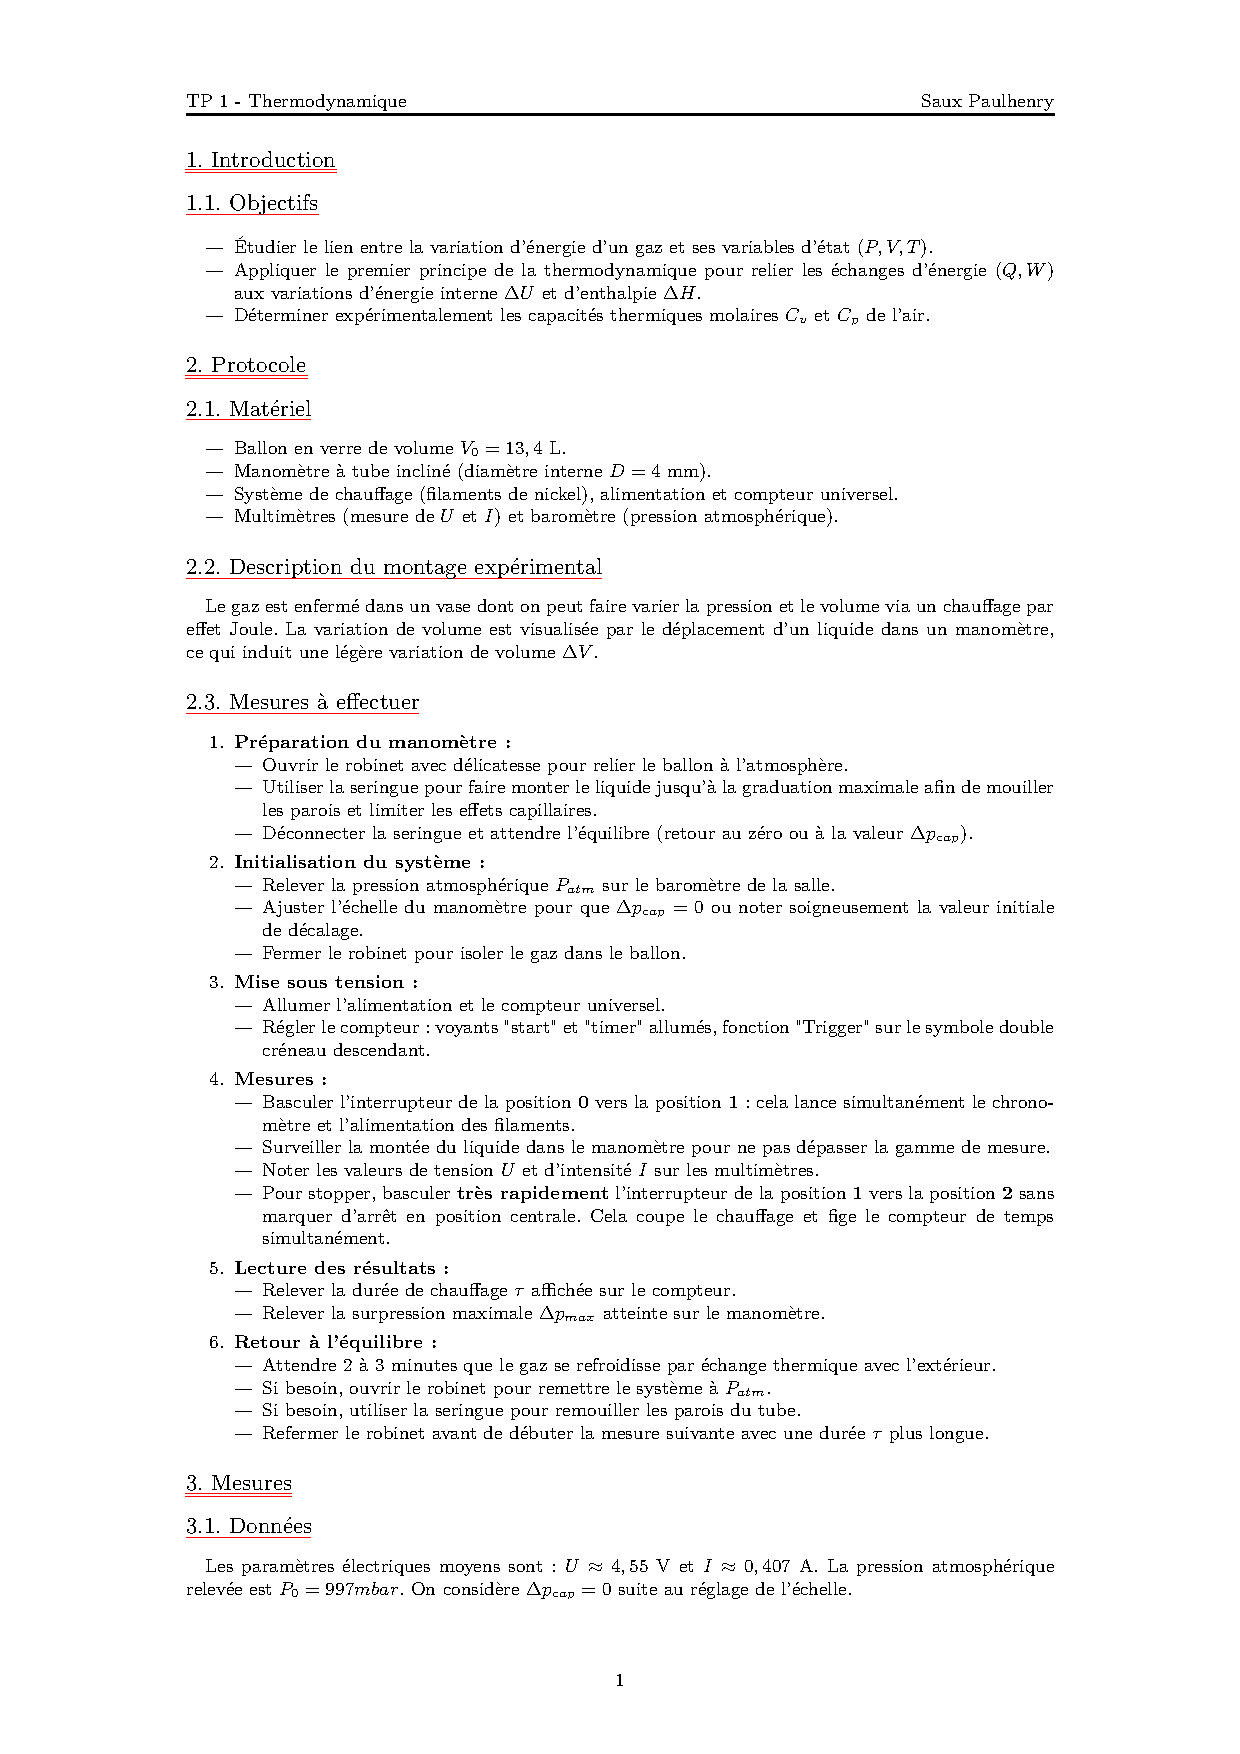
\includegraphics[scale=0.4]{thermo1}
 \end{center}
\caption{Évolution de l'énergie interne (en bleue) et de l' enthalpie (en rouge) en fonction de $\Delta pV$}
\end{figure}


\section{Exploitation des résultats}
\subsection{Expressions théoriques}
\begin{itemize}
    \item \textbf{Variation de volume} : $\Delta V = S \cdot x = \frac{\pi D^2}{4} \cdot x$. Avec $D=4$mm, $\Delta V$ est proportionnel à la graduation lue sur le manomètre. On sait qu'une longueur de 140mm correspond à 2 mbar, donc $x=70\cdot \Delta p$.
    \item \textbf{Variation de PV} : $\Delta(PV) = P_{max}V_{max} - P_0V_0 = P_0 \Delta V + V_0 \Delta p + \Delta p\Delta V$.
    \item \textbf{Chaleur injectée} : $Q_i = U \cdot I \cdot \tau$.
    %\item Variation de pression : $\Delta p_{max} = 
    \item \textbf{Travail} : $W = - \int P_{ext}\mathrm{d} V =  -P_{atm} \Delta V$ (le gaz pousse la colonne de liquide contre la pression extérieure, qui est constante et vaut $P_0$).
\end{itemize}

\subsection{Énergie interne et Enthalpie}
D'après le premier principe, $\Delta U = Q + W$. Pour un gaz parfait, $U$ ne dépend que de $T$\footnote{D'après la 1ère loi de Joule}, soit $\Delta U = n C_v \Delta T$. Comme $PV = nRT$, on a $\Delta(PV) = nR\Delta T$, d'où :
$$ \Delta U\footnote{Correspond à Y1} = \frac{C_v}{R} \Delta(PV) $$
De même pour l'enthalpie : $\Delta H\footnote{Correspond à Y2} = \Delta U + \Delta(PV) = \frac{C_p}{R} \Delta(PV)$.


\subsection{Calcul des capacités thermiques}

L'exploitation des courbes de tendance sur Regressi nous donne les pentes expérimentales suivantes :
\begin{itemize}
    \item Pente de la droite $Q_i + W = f(\Delta PV)$ : $a_1 = 3,40\pm0,040$
    \item Pente de la droite $Q_i + W + \Delta(PV) = f(\Delta PV)$ : $a_2 = 4,40\pm0,040$
\end{itemize}

D'après les relations établies précédemment, ces pentes correspondent respectivement aux rapports $C_v/R$ et $C_p/R$. En utilisant la constante des gaz parfaits $R = 8,314$ J.mol$^{-1}$.K$^{-1}$, nous en déduisons les capacités thermiques molaires expérimentales de l'air :

\begin{itemize}
    \item $C_v = a_1 \cdot R = 3,40 \times 8,314 \approx 28,27$ J.mol$^{-1}$.K$^{-1}$
    \item $C_p = a_2 \cdot R = 4,40 \times 8,314 \approx 36,58$ J.mol$^{-1}$.K$^{-1}$
\end{itemize}

\subsubsection*{Vérification de la relation de Mayer}
La relation de Mayer pour un gaz parfait impose que $C_p - C_v = R$, soit $\frac{C_p - C_v}{R} = 1$. 
Expérimentalement, nous observons :
$$a_2 - a_1 = 4,40 - 3,40 = 1,00$$
La relation de Mayer est donc vérifiée avec une excellente précision, ce qui valide l'approximation de l'air comme un gaz parfait dans les conditions de l'expérience.

\subsubsection*{Calcul du rapport des capacités thermiques $\gamma$}
Le coefficient adiabatique $\gamma$ est défini par le rapport $C_p/C_v$ :
$$\gamma = \frac{a_2 \cdot R}{a_1 \cdot R} = \frac{4,40}{3,40} \approx 1,29$$

\subsubsection*{Commentaires}
La valeur théorique pour l'air (considéré comme un gaz diatomique) est $\gamma_{théo} = 1,4$. Notre valeur expérimentale de $1,29$ est légèrement inférieure. 

Cette différence est supérieure à l'incertitude de mesure $U(\gamma)$.

Ce décalage s'explique par les pertes thermiques au cours du chauffage : une partie de l'énergie électrique injectée par effet Joule est dissipée vers les parois du ballon en verre plutôt que de servir uniquement à l'élévation de température du gaz. Cela augmente artificiellement les valeurs de $Q_i$ mesurées pour une variation $\Delta(PV)$ donnée, et donc la valeur des pentes.
\section{Conclusion}
L'expérience a permis de quantifier les transferts énergétiques lors du chauffage. L'écart entre les valeurs expérimentales et théoriques de $\gamma$ s'explique par les pertes thermiques à travers les parois du vase en verre, qui ne sont pas parfaitement adiabatiques.

\end{document}
